\documentclass[12pt, a4paper]{memoir} % for a short document
\usepackage[english]{babel}
\usepackage [vscale=0.76,includehead]{geometry}              
\usepackage{fullpage}
\usepackage{mathptmx} % font = times
\usepackage{helvet} % font sf = helvetica
\usepackage[latin1]{inputenc}
\usepackage{relsize}
\oddsidemargin 0.0cm  
\evensidemargin 0.0cm  
\textwidth 17cm 
\topmargin -1cm 
\textheight 23.5cm
\usepackage{graphicx}
\usepackage{float} 
\usepackage{multimedia}
\usepackage{amsmath,amssymb}
\usepackage{listings}
\usepackage{graphicx} % Allows including images
\usepackage{booktabs} % Allows the use of \toprule, \midrule and \bottomrule in tables
%\usepackage[nottoc, notlof, notlot]{tocbibind}
\usepackage{amsfonts}
\usepackage{amsmath,bm}
\usepackage{hyperref}
\usepackage[round]{natbib}
\lstset{
  numbers=left,   
  firstnumber=1,
  numberfirstline=true,
  language=C, 
  frame=L
  } 



\bibliographystyle{plain}

%\headstyles{komalike}
\nouppercaseheads
\chapterstyle{dash}
\makeevenhead{headings}{\sffamily\thepage}{}{\sffamily\leftmark} 
\makeoddhead{headings}{\sffamily\rightmark}{}{\sffamily\thepage}
\makeoddfoot{plain}{}{}{} % Pages chapitre. 
\makeheadrule{headings}{\textwidth}{\normalrulethickness}
%\renewcommand{\leftmark}{\thechapter ---}
\renewcommand{\chaptername}{\relax}
\renewcommand{\chaptitlefont}{ \sffamily\bfseries \LARGE}
\renewcommand{\chapnumfont}{ \sffamily\bfseries \LARGE}
\setsecnumdepth{subsection}


% Title page formatting -- do not change!
\pretitle{\HUGE\sffamily \bfseries\begin{center}} 
\posttitle{\end{center}}
\preauthor{\LARGE  \sffamily \bfseries\begin{center}}
\postauthor{\par\end{center}}

\newcommand{\jury}[1]{% 
\gdef\juryB{#1}} 
\newcommand{\juryB}{} 
\newcommand{\session}[1]{% 
\gdef\sessionB{#1}} 
\newcommand{\sessionB}{} 
\newcommand{\option}[1]{% 
\gdef\optionB{#1}} 
\newcommand{\optionB}{} 

\renewcommand{\maketitlehookd}{% 
\vfill{}  \large\par\noindent  
\begin{center}\juryB \bigskip\sessionB\end{center}
\vspace{-1.5cm}}
\renewcommand{\maketitlehooka}{% 
\vspace{-1.5cm}\noindent
\includegraphics[height=14ex]{logoINP.png}\hfill\raisebox{2ex}{
\includegraphics[height=7ex]{logoUJF.jpg}}\\
\bigskip
\begin{center} \large
Master of Science in Informatics at Grenoble \\
Master Math\'ematiques Informatique - sp\'ecialit\'e Informatique \\ 
option \optionB  \end{center}\vfill}
% End of title page formatting

\option{$<$GVR$>$}
\title{ Inverse Procedural Generation of Geological Stories}%\\\vspace{-1ex}\rule{10ex}{0.5pt} \\sub-title} 
\author{Garcia Maxime}
\date{ $<$June 23rd 2016$>$} % Delete this line to display the current date
\jury{
Research project performed at $<$INRIA Monbonnot$>$ \\\medskip
Under the supervision of:\\
$<$Dr. R\'emi Ronfard ,INRIA$>$\\\medskip
Defended before a jury composed of:\\
$[$Prof/Dr/Mrs/Mr$]$ $<$first-name last-name$>$\\
$[$Prof/Dr/Mrs/Mr$]$ $<$first-name last-name$>$\\
$[$Prof/Dr/Mrs/Mr$]$ $<$first-name last-name$>$\\
$[$Prof/Dr/Mrs/Mr$]$ $<$first-name last-name$>$\\
}
\session{$[$June$]$\hfill 2016}

\begin{document}
\selectlanguage{english} % french si rapport en français
\frontmatter
\begin{titlingpage}
\maketitle
\end{titlingpage}

Abstract

In this project we tackle the problem of restoring the complete history of a 2D geological 
subsurface. It is represented by a 2D sketch and we will produce a backward animation, starting
at the section current state going in the past while detecting and un-doing geological events
that possibly occured throught its history. Several scenarios will be taken into account while keeping
only the most plausible ones. The animation is the result of running a simulation using mass spring
systems mapped on nthe different part of the cross-section.

I) Introduction

Hand-drawn sketches are useful in geology for illustrating and validating hypotheses. 
For instance they can be used to reconstruct a 3D view of the subsurface by drawing a 2D top view of the current terrain (2) or 2D vertical cross-sections. 
Futhermore they can also be used to restore the subsurface history using 2D slices (vertical cross-sections) Moreover by analysing the different layers and faults, the geologist is able to reconstruct the geometrical evolution specially provoqued by compression or extension of the rock masses before, after or during deposit and erosion of the sediments and basement rocks. 
The resulting drawing is called a restoration (ref) (a single of sequential geometric description of the cross-section).
However those drawings are rather limited. On top of representing only one 2D cross-section of the terrain being investigated, they can only represent hypotheses on the underground geometry at discrete time steps, rather than a complete continuous history. In addition insuring consistency between these sketches over time heavily depends on available data, maturity of the regional geological interpretation and the skills of the geologist, i.e. his knowledge on the way rocks and sediments fold, on the way faults propagates and produce sliding and displacements, and on the way sediments are deposited or eroded, etc...
Building, Exploring and comparing different hypotheses of kinematic restoration is very difficult, if not impossible, with the current pipeline (workflow). 
Recently, it was proposed to organize geological sketches into story trees to present and compare different interpretations of the formation of a given terrain (6) but the task remains labor-intensive, requiring the geologist to draw every sketch in the story tree. Moreover, even while being skillful and experienced, it’s hardly impossible to a geologist to express a continuum of the deformation of a geological cross-section with available tools.
In this internship, we would like to follow up on this line of research by proposing methods for inferring a geological story tree directly from very few geological sketches, and presenting the resulting tree of possible geological stories as an animation.


II) State of the Art

Like mentioned above, several continuous animation tools for subsurface evolution over time are already available. They work on the assumption that sedimentary layers were in a horizontal configuration at the starting position which is a well used hypothesis in geology. With this assumption and using the Coulomb prism theory (ref) sofware such as SLAMTec or OptumG2 (refs ?) offer the possibility to mechanically simulate the compression of a geological cross-section.
The goal of this kind of forward simulation is to validate a restoration that had been generated from a present dating 2D section and see if the result matches with it. This kind of simulation is configurable by several parameters such as the erosion and the friction coefficients.
Geological cross-section restoration can be obtained thanks to geometrical tools (refs ?). Those tools deal with each block (soil section between two faults) one by one and flatten each layer while conserving their respective area or length. After the flattening operation the user can manually stick the new block to its neighbours with the corresponding layers facing each other. Here is an example of restoration taken from Chartreuse slice:

III) Geological Structure Representation and Analysis
	How do we represent a Cross Section.
	A Cross-Section contains several parts : 
		-It contains parts of geological layers => floors or moduli
		- A geological layer is a layer composed of the same kind of material.
		In our case we deal with sementary layers. It implies that each material is caracterized by its temporal existance.	
	   	- Faults which can be seen as discontinuities in the XS
		- Blocks which represent the groups of floors delimited by faults.
		- Each Material is caracterised by a Young Modulus which describe its plasticy and elesticity,
		an age period and a friction coefficient.

Drawing analysis. As Mentionned before our input is a colored vpaint drawing which is composed of face, edges and vetices stored in 
a vertex complex graphics strucutre (ref). Passage du sujet.
In the drawing we color faces which represent the different moduli of the XS with the color being its material. moduli of the same color have the same material, therefore they belong to the same layer. We represent interlayers by a white edge while the other contour egades are black. Gaps inside a block are also represented in white and are automatically detected as gaps meaning that erosion impacted this region for sure. line could be added to give hint on the rosion.

Then we have to extract the structure out of this drawing. Meaning that we have to identify the different blocks, moduli, faults and materials from the drawing. To do so we proceed this way: the vpaint output format is an xml file which describe our drawing in terms
of faces, edges and vertices. Each faces has a cycling orientation which is clockwise or counterclockwise but for building and manipulating our structure more easelly we choose that all of our layer will be first read clockwiselly and from the most recent (the higher in general) to the oldest. In fact it is an easy task to wirte the layers in the correct way but we need to find out which layers belong to the same block. To solve this issue we will use the interlayers and then the white edges. Two layers belong to the same block if they share a commun white edge. Thanks to this method we build our blocks. we can notice that the youngest and the oldest layer have just one interlayer that make them part of a block. However we will describe our layer with four part of the contours the upper interlayer, the righedges, the bottom interlayer and the left edges. Consequently for these two specific layer we will compute automatically the lacking interlayer (limitation it is not always good).
	

IV) Story Telling

As we mentionned before, geologist are usually able to restore the history of the cross section by using several geometrical and simulation tools.
However then only get one final state of the section whcih represents what was the XS before any techtonic movement. Here we are interested in what 
happened between today XS and the restoration. Indeed most of the time there are several scenarios that lead the initial state to the restoration.
This is what we want in this project. We want to explore the most plausibles scenarios and see the resulting animation of exploration.
To do so we wiil propose to the user to undo geological events at each time step. We can count already five events to undo : faults, erosion, sedimentation, folding and compaction. Those event will be automatically detected and resbored. In order to solve the issue properlly we'll use two graphs:
	-Story graph
	-Event graph

The Story graph represents the event paths we can run the simulation on. a node represents the list of event we can simulate at time t and an edge represents the event simulated between two nodes. Event graph used in the creation of this graph. It is the graph the user will explorer to see the animation of as many scenarios he wants to see.

Each event has a pre condition and and postcondition and will finish in a state.
Also a event can be have the special property to be dynamic meaining that it will be created during the simulation and not at 
the graphs creation.

The event graph shows time dependencies between geological events. An event is represented by a node and an edge represents a dependency. It is also computed automatically but it can be edited using information provided by the user. Has it contains only dpendencies

Only 4 out of the 5 event have been treated, the compaction will be reserved for later.
Describe the 4 events:


Faults: subdivided into modulus event
	Our XS contains what is called fault which corresponds to the breaking of a block into two parts and only two parts. Geologically speaking when a fault begin to open, it splits the block starting by the oldest moduli that is to say from bottom to up. 
	
	We will use this property to decompose our un fault event into several stickModulus events. As we just said the fault split the block into two parts (which are new blocks) and one part is inevitably above the other in terms of y coordinates. Meaning that the corners of each modulus of the upper block is higher than the respecting corners of each modulus of the lower block (see the exemple below). 
	
	As a result the modulus event will correspond to applying forces to the lower block in order to unfold it and make the upper modulus converging to the respecting modulus and then stick together the two moduli when they face each other in terms of y coordinates.
	
	Once all moduli event have ended the fault event can end as well.
	
	The preconditions are:
	
	The posconditions are:

Erode: three types of erosion

Sediment:

	The preconditions are: if we un sediment one material in all the blocks
	we all the material younger that this one should ahve been unSedimented already. If it is just one molulus we should also check if inside its block there are  no modulus with a material younger than the material of the modulus we want to unSediment.
	
	the postconditions are: the un sedimentation has a duration htat should comes to an end to finish and at the end of the time the concerned moduli should have been erased from the XS. also the massSpring mesh should be reGenerated at the end of the event in order to uniformise the new state of the XS.

Fold:
	The preconditions are: there are no precondition for this event. the user is free to play with this event as it allows geologists to test their hypothesis on forces that have been applied to the XS in the past and with a duration.
	
	The posconditions are: the event no longer apply forces on the concerned particles
	


V) Simulation

\section{General Overview}

Here we will present our first method to tackle the problem of proposing a panel of plausible animations giving geological restoration as final state from a 2D input slice. 
The main idea of our methods is to map a mass spring system on each block (section between two or several faults) of the slice and simulate a extension by freezing the physics of several blocks at each time step and let the others move as they should given geological events. The output of our method we will a series of inbetween VGC which will be played on VPaint.\\\\
The first step of our method is to draw the 2D slice using VPaint which allow the user to do it pretty quickly.
This drawing will highlight all the different blocks which are contained in the slice.
In addition the VPaint drawing will show all the different layers of each block and faults. Additionnal information such as erosion lines can be added. \\\\
After drawing our section in VPaint we will read the .vec file in our GeoPaint editor in order to add all the necessary information about our section such as the layers' materials containing crutial information (density, age, etc...) or even  additionnal information about faults and erosion lines. This information will allow us to run the animation over our section.
Indeed once the geo editing is finished we will gather all the information into one format (.geo) and will use it to describe our slice and animate it.\\\\
The first step for animating is mapping a mass-spring system into each block. Then we have to solve the restoration problem at a geological point of view, that is to say build the first story tree and find a method to propose which event can happen at each node.\\\\
As the first proposed story tree is computed fully automaticaly it may not show the most plausible result that's why we propose the user to choose events a list of plausible geological events at each node.
This way the user can construct all the plausible stories he wants.

\section{General structure}
One important matter in our model is to choose carefully the representation of our slices as it will affect how we will animate it.
We choose one possible representation of a geological slice but we are aware that some part of this structure can be modified through the project progression.\\\\
Similary to the drawing a slice is composed of blocks, faults and erosion lines. It also contains a list of all the materials composing the different layers.This list will be usefull when we want to see if one material disappeared from one block. Each blocks is composed of layers and interlayers lines. Knowing all the interlayers is important to link the layer mapping together (see Animation Model section).\\\\
Each block contains a list of the materials composing its layers. Like said abbove we will compair it to the slice material to take into account erosion effect which cause layers to disappear. \\\\
Each layer contains its interlayers,left and right sides and also its corners which are important for linking blocks together during the animation. The layer contains also its material which gives a lot information for the animation (density, friction, erosion speed, sedimentation speed). 
In fact this information will be taken into consideration inside the mass spring system attached to the layer.
Each fault contains each line composing it. Sub faults which we know that came after an other can be added.


\section{Animation Model}

Like mentionned above the animation will be done by mapping a mass-spring system on each block. In fact it is more accurate to say that mass-spring system are mapped on layers instead of blocks. We proceed this way to take into account each layer orientation in the mapping as it is mapped according to layer's borders gradients. Considering that each layer is a rectangle that underwent some deformations the mapping will be done following the steps:	\\\\		
\indent	- First we have to put the masses both at the layer border but also inside it.\\\\
\indent	- We put the masses on the borders in an uniform way.\\\\
\indent	- We put the masses inside the layer: to do so we have two solutions:\\\\
\indent \indent	- Compute hermite curve between each pair mass of the two interlayer and place particles uniformly on those curves.\\\\
\indent \indent	- Compute the intersections between the previous hermite curves and the  one coming from each pair mass of the two sides and place particles at those intersections.\\\\
	Even if the second solution might show better results that the first one we have chance that the curve comming from the sides might be not inside the layer due to big deformation making the layer non convex. \\With the first solution this problem is unlikely to occur because of the type of the deformations. In either case the hermite curves be created using a mass pair and the gradient of the broder at each extremity as tangents. This way the layer will tend to transform back to a rectangle shape.\\\\
\indent	- Link particles with springs. \\We divide springs into 5 categories like described in \citep{cloth}: Vertical, Horizontal, DownShear, UpShear and Flexion. Adding flexion spring show better results in terms of shape preservation and breaking prevention. The resulting network looks like:\\
	
	\begin{figure}[H]
	\centering
	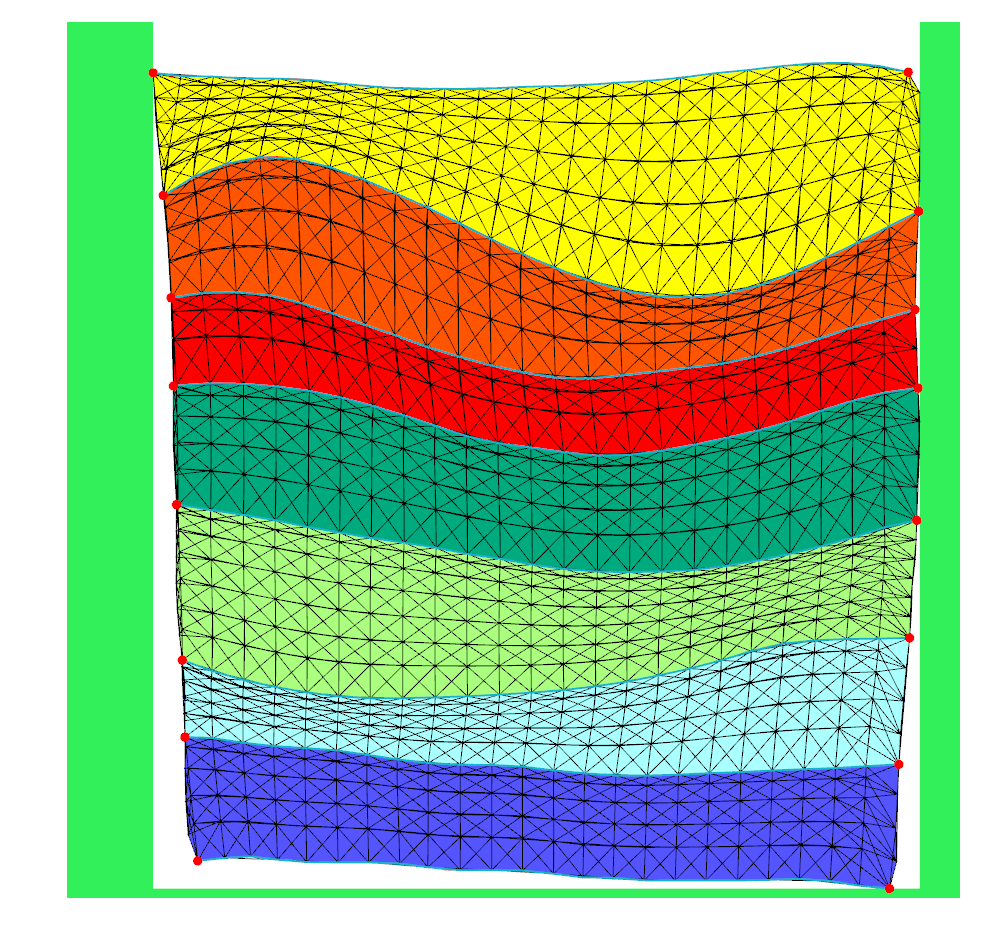
\includegraphics[scale=0.5]{springMapping.png}
	\caption{Mass-Spring Mapping on a layer. In purple: interlayers. In white: sides}
	\end{figure}
	
	
\indent	- The springs we use will also have a torsion resistance in order to accentuate the shape change of the layer.\\\\
In terms of physical equations for a single mass spring system we use the implicit euler scheme and algorithm descibed in \citep{caltech}. We use this scheme instead of an explicit one because it is proven to be more stable with big time step ($dt = 0.02$).\\\\ 
Each particle has the same mass $m$ and possesses at step $n$:\\\\
\indent	- A position  $x_i^n$\\\\
\indent	- A speed $v_i^n$ \\\\\
\indent	- Applied forces $F_i^n$ (containing filtered, corrected and external forces).\\\\
At each time step we will solve the second Newton's law:\\

\begin{align}
	v_i^{n+1} &= v_i^n + F_i^{n+1} \frac{dt}{m}\\
	x_i^{n+1} &= x_i^n + v_i^{n+1} dt 
\end{align}

with:

\begin{equation}
F_i^{n+1} = - \sum\limits_{j|(i,j)\in Edges} k_{ij}(x_i - x_j) + k_{ij}l_{ij}^0\frac{(x_i - x_j)}{||(x_i - x_j)||}
\end{equation}


For each particle we want to integrate the above equations. The problem is that we don't know the forces at step $n + 1$ as we don't know the position of the particles at this step. That is why we use a first order approximation to solve the problem at step $n + 1$:

\begin{equation}
	F^{n+1} = F^n + \frac{\partial F}{\partial x}(x^{n+1} - x^n)
\end{equation}

\noindent Thus we need to compute $H =  \frac{\partial F}{\partial x}$ which is the Jacobian of $F$.\\\\
\noindent By using (1) and (4) we have the following result:
\begin{align*}
	(x^{n+1} - x^n) &= (v^n + (v^{n+1} - v^n))dt \\
	(v^{n+1} - v^n) &= (I - \frac{dt^2}{m}H)^{-1}(F^n + dt H v^n)\frac{dt}{m}
\end{align*}

We now have approximated our equations into a solvable system and we can notice that an additionnal force came from this approximation $dt H v^n$ . It is an implicit viscosity that takes into account the movement of the neighbouring particles.
Consequently we have for each particle $i$ a new force:

\begin{equation}
\tilde{F_i} = k dt \sum\limits_{j|(i,j)\in Edges}(v_j - v_i)
\end{equation}


The last thing to compute is $H$. Like in \citep{caltech} we will approximate $H$ by just integrating the linear part of the elastic force which is equal to:

\begin{equation}
F_{(i,j)} = -k_{ij}(x_i - x_j) + k_{ij}l_{ij}^0\frac{(x_i - x_j)}{||(x_i - x_j)||}
\end{equation}

If $H$ represents only the Jacobian of $F = -k_{ij}(x_i - x_j)$ it has the form:\\
\begin{center}
$
\left\{
\begin{array}{ll}
H_{ij} &= k_{ij} if i \neq j \\
H_{ii} &= -\sum\limits_{j \neq i}k_{ij}
\end{array}
\right.
$
\end{center}

Integrating only the linear part implies that we will have some error at the end of the integration. However we can notice that the non linear part $k_{ij}l_{ij}^0\frac{(x_i - x_j)}{||(x_i - x_j)||}$ has a constant magnitude during the simulation between two steps, so this force just implies a rotation that we will compensiate with another force. Thus we will correct the angular momentum $\delta T$ introduced by this method by adding correcting forces:
\begin{align*}
\delta T &= \sum\limits_{i=1}^n (x_G - x_i)\wedge F_i^{filtered} \\
F_i^{corrected} &= (x_G - x_i)\wedge \delta T dt
\end{align*}

with:
\begin{equation}
F_i^{filtered} = \sum\limits_{i=1}^n F_{ji}W_{ij}
\end{equation}

However in our case the equilibrum length of the springs will change over time creating an error in the angular momentum but we will try compensating this with torsion forces.\\\\

Finally we add torsion forces as external forces (along with gravity) because it is a non linear force and we can't integrate it:

\begin{equation}
F_{ij}^{torsion} = -k_{torsion}\Delta \theta \vec{n}
\end{equation}

with $\Delta \theta$ being the angle between a unit vector depending on the spring type (Vertical, Horizontal, DownShear or UpShear) and the vector $x_i - x_j$. $\vec{n}$ is the normal vector to $x_i - x_j$ pointing toward the unit vector.\\\\
Having this physical structure we will simulate extension and take into account geological features. For the moment we assume that the density and the spring stiffnesses (elastic and torsion) are proportionnal. The friction coefficient will directly be taken into account in the collision computation between faults and particles. As for erosion and sedimentation we will add or remove partcle in the mass-spring system to simulate those events.\\\\
Regarding the extension simulation we will first pull the side where the extension has to occur. This is known before simulating because it is provided by the user. At each time step we will freeze the animation of all the blocks, translate them toward extension apply the physics only to the blocks which are considered to move. The blocks moving undergo either discrete geological event (such as fault) or/and continuous event (erosion or sedimentation). When solving fault apparition we have to stick blocks together. This will be done by attaching corners of the layers when the matching ones are near each other enough. When all the corners are matched we have a new block where we must recompute a new mass spring system.\\\\
Computing a mass spring system can take some time (few seconds for big systems) and can be noticable especially during block fusion but that is not a problem because the goal of the project is to record at each time step the result of our simulation as an inbetween vac which can be played fluently.\\\\


VI) Results

VII) Conclusion

glossary
	
Faults: extensive, inverse (compress), décrochement

Floor, Modulus.

Blocks;

Cross section, 2D slice.

Material.

Young Modulus.

Event: unFolding, unErode, unSediment, un


\bibliography{pfe.bib}

\end{document} 